\documentclass[twocolumn,prl,showpacs,superscriptaddress]{revtex4-1}   % use preprint or twocolumn
%\usepackage{geometry}                % See geometry.pdf to learn the layout options. There are lots.
%\geometry{letterpaper}                   % ... or a4paper or a5paper or ...
%\geometry{landscape}                % Activate for for rotated page geometry
%\usepackage[parfill]{parskip}    % Activate to begin paragraphs with an empty line rather than an indent
\usepackage{graphicx}
\usepackage{amsmath}
\usepackage{amssymb}
\usepackage{epstopdf}
\usepackage{dcolumn}% Align table columns on decimal point
\usepackage{bm}% bold math
\usepackage{verbatim}
\usepackage{amsfonts}
\usepackage{cancel}
\usepackage[utf8]{inputenc}
\usepackage{graphicx}
\usepackage{setspace}
\usepackage{tabularx}
\usepackage[export]{adjustbox}



\DeclareGraphicsRule{.tif}{png}{.png}{`convert #1 `dirname #1`/`basename #1 .tif`.png}


\newcommand{\sspace}{$\enspace$}
\newcommand{\ssspace}{$\quad$}
\newcommand{\proofend}{\mbox{ }\hfill$\Box$\\}
\newcommand{\ddf}[2]{\frac{\mathrm{d} #1}{\mathrm{d} #2}}
\newcommand{\pdf}[2]{\frac{\partial #1}{\partial #2}}
\newcommand{\ee}[1]{\cdot 10^{ #1}}
\newcommand{\bra}[1]{\left\langle #1 \right|}
\newcommand{\ket}[1]{\left| #1 \right\rangle}
\newcommand{\brakett}[3]{\left\langle #1 \right|#2\left| #3 \right\rangle}
\newcommand{\braket}[2]{\left\langle #1 \right|\left. #2 \right\rangle}
\newcommand{\trace}[1]{\mathrm{Tr}\left(#1\right)}
\newcommand{\abs}[1]{\left|#1\right|}
\newcommand{\figref}[1]{Fig. \ref{#1}}
\newcommand{\eqnref}[1]{Eqn. \eqref{#1}}

\newcommand{\ak}{\alpha_{\textrm{K}}}
\newcommand{\arb}{\alpha_{\textrm{Rb}}}
\newcommand{\acs}{\alpha_{\textrm{Cs}}}

\newcommand{\polK}{42.97(2)(8)}
\newcommand{\polRb}{47.44(3)(9)}
\newcommand{\polCs}{59.45(3)(11)}
\newcommand{\polKSysOnly}{42.97(8)}
\newcommand{\polRbSysOnly}{47.44(9)}
\newcommand{\polCsSysOnly}{59.45(11)}

\newcommand{\ratRbK}{1.1040(9)}
\newcommand{\ratCsK}{1.3835(9)}
\newcommand{\ratCsRb}{1.2532(10)}

% obselete
\newcommand{\sigv}{ASDFASDFASDF}
\newcommand{\sigr}{ASDFASDFASDFA}

\newcommand{\Omegalab}{\Omega_{\mathrm{lab},y}}

\newcommand{\dphisep}{\Delta\Phi_{\mathrm{sep}}}
\newcommand{\dphisepj}{\Delta\Phi_{\mathrm{sep},j}}

\newcommand{\dphisag}{\Delta\Phi_{\mathrm{sag}}}
\newcommand{\dphiaccel}{\Delta\Phi_{\mathrm{accel}}}

\newcommand{\cenv}{C_{\mathrm{env}}}

\newcommand{\rcs}{\mathcal{R}_{\mathrm{Cs}}}

\newcommand{\etal}{\textit{et al.}}
\newcommand{\etalspace}{\textit{et al. }}

\newcommand{\AAA}{\mathrm{\AA}}




\begin{document}

%\title{Improved Absolute and Ratio Measurements of Ground-State Polarizabilities of Cs, Rb, and K using Atom Interferometry}
\title{Measurements of the Ground-State Polarizabilities of Cs, Rb, and K using Atom Interferometry}

\affiliation{Department of Physics, University of Arizona, Tucson, AZ 85721}
\affiliation{College of Optical Sciences, University of Arizona, Tucson, AZ 85721}
\author{Maxwell D. Gregoire}
\affiliation{Department of Physics, University of Arizona, Tucson, AZ 85721}
\author{Ivan Hromada}
\affiliation{Department of Physics, University of Arizona, Tucson, AZ 85721}
\author{William F. Holmgren}
\affiliation{Department of Physics, University of Arizona, Tucson, AZ 85721}
\author{Raisa Trubko}
\affiliation{College of Optical Sciences, University of Arizona, Tucson, AZ 85721}
\author{Alexander D. Cronin}
\affiliation{Department of Physics, University of Arizona, Tucson, AZ 85721}
\affiliation{College of Optical Sciences, University of Arizona, Tucson, AZ 85721}
\email{cronin@physics.arizona.edu}
\homepage{http://www.atomwave.org}

\date{\today}





\begin{abstract}
We measured the ground-state static electric-dipole polarizabilities of Cs, Rb, and K atoms using a three-nanograting Mach-Zehnder atom beam interferometer. Our measurements provide benchmark tests for atomic structure calculations and thus test the underlying theory used to interpret atomic parity non-conservation experiments. We measured $\acs = 4\pi\epsilon_0 \times \polCsSysOnly \AAA^3$, $\arb = 4\pi\epsilon_0 \times \polRbSysOnly \AAA^3$, and $\ak = 4\pi\epsilon_0 \times \polKSysOnly \AAA^3$. We report ratios of polarizabilities $\acs/\arb = \ratCsRb$, $\acs/\ak = \ratCsK$, and $\arb/\ak = \ratRbK$ with smaller fractional uncertainty because most of the systematic error is correlated among measurements. 
Since Cs atom beams have shorter de Broglie wavelengths, we developed measurement methods that do not require resolved atom diffraction patterns.
Specifically, we used phase choppers to measure atomic beam velocity distributions, and we use electric field gradients to shift the interference patterns' phase proportional to atomic polarizability.
\end{abstract}





\maketitle



\begin{figure*}
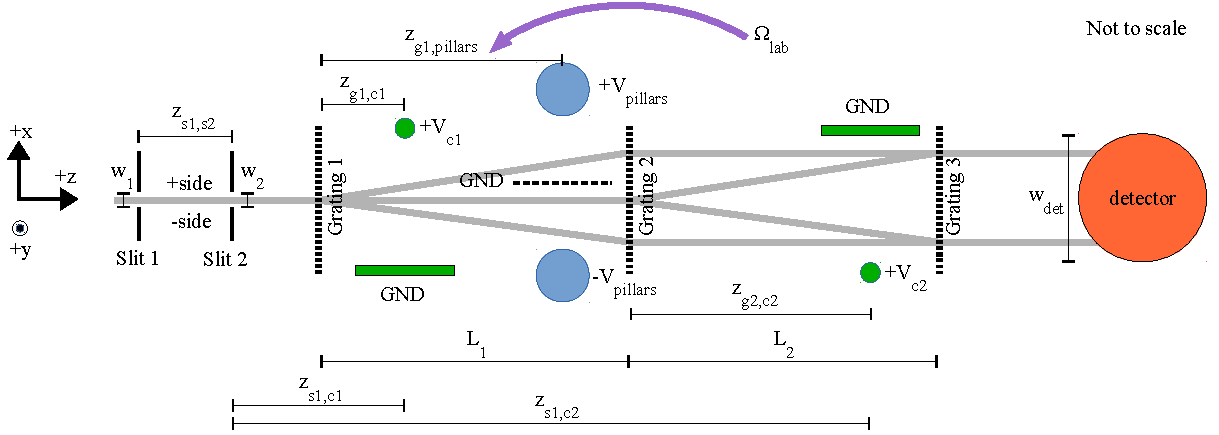
\includegraphics[width=\linewidth,keepaspectratio]{IFM_diagram1.pdf}
\caption{\label{IFMDiagram}(Color online) Diagram of the atom interferometry apparatus. Dimensions are given in red.  The supersonic atom beam is collimated by two slits s1 and s2 with widths $w_1$ and $w_2$ before entering the three-grating Mach-Zehnder interferometer. 
The gratings, g1, g2, and g3, are spaced longitudinally such that $L_1 = L_2$, which causes an interference pattern forms at the position of the g3.
Due to the rotation of the Earth, the lab has a rotation rate about the vertical axis of $\Omegalab = 38.88$ $\mu$rad/s. 
The pair of blue circles represents oppositely-charged cylindrical electrodes (extending perpendicular to the page) that form a virtual ground plane between them. The electric field from these electrodes polarizes the atoms and thereby shifts the interference pattern's phase. 
The phase choppers are shown in green; each phase chopper is a charged wire next to a grounded plane. The geometry terms relevant to the pillars and phase choppers are displayed in \figref{EDiagram} and discussed in section II.a. Dimensions are given in Table \ref{tableDimensions}.}
\end{figure*}

\section{I. Introduction}

High-precision measurements of static electric-dipole polarizabilities serve as benchmark tests for \textit{ab initio} calculations of electric-dipole transition matrix elements. 
These calculations require understanding quantum many-body systems with relativistic corrections, and there are many different methods that attempt to calculate these matrix elements in a reasonable amount of computing time \cite{Mitroy2010}. Testing these methods is important because these matrix elements are used to calculate many atomic properties.
Measuring alkali static polarizabilities as a means of testing atomic 
structure calculations has been of interest to the physics community since
1934 \cite{Scheffers1934}, and has been
accomplished using deflection \cite{Scheffers1934,Chamberlain1963,Hall1974,Ma2015}, the E-H gradient
balance technique \cite{Salop1961,Molof1974a}, time-of-flight measurements of atoms in a fountain \cite{Amini2003},  and atom interferometry 
\cite{Ekstrom1995,Miffre2006,Holmgren2010}.

We measured the static electric-dipole polarizabilities of K, Rb, and Cs atoms with 0.19\% uncertainty using a Mach-Zehnder three-grating atom interferometer \cite{Berman1997,Cronin2009} with an electric field gradient interaction region. We used the same apparatus for all three atomic species, so we can also report polarizability ratios with 0.08\% uncertainty because many sources of uncertainty are correlated between measurements of different atoms. 

We also compare our measurements to polarizability values of similar uncertainty deduced from studies of atomic lifetimes, Feshbach resonances, and photoassociation specroscopy. Then we analyze our measurements to report the Cs $6p_{1/2}$ and $6p_{3/2}$ state lifetimes, Rb $5p_{1/2}$ and $5p_{3/2}$ state lifetimes, and K $4p_{1/2}$ and $4p_{3/2}$ state lifetimes, as well as the associated principal electric dipole matrix elements, oscillator strengths, and line strengths. 
We also use our $\acs$ measurement to report the Cs van der Waals $C_6$ coefficient,
and we combine our measurements with recent measurements of 
transition Stark shifts to report some excited state polarizabilities with better than 0.09\% uncertainty.

Testing Cs atomic structure calculations by measuring $\acs$ is particularly important for parity non-conservation (PNC) research, which places constraints on beyond-the-standard-model physics. The coupling strength, $E_{\mathrm{PNC}}$, of $Z^0$-mediated interactions between the Cs chiral, valence electron and nuclear neutrons can be written in terms of the electric dipole transition matrix elements and the nuclear weak charge parameter $Q_W$. Researchers can use atomic structure calculations to deduce a value of $Q_W$ from an $E_{\mathrm{PNC}}$ measurement \cite{Cho1997} to compare to the $Q_W$ predicted by the standard model \cite{Bouchiat1999,Dzuba2012}. Our measurement of $\acs$ tests the methods used to calculate the relevant matrix elements and provides a benchmark for the $\brakett{6s_{1/2}}{\hat{D}}{6p_{1/2}}$ matrix element, one of the terms in the expression for $E_{\mathrm{PNC}}$.

To our knowledge, this is the first time atom interferometry has been used to measure Cs polarizability. Measuring polarizability by the method described here requires precise measurement of our atom beam's velocity distribution. Because it is challenging to obtain resolved diffraction with a 1500 m/s Cs beam, we did not measure its velocity using diffraction as was done by Ekstrom \etalspace and Holmgren \etalspace \cite{Ekstrom1995,Holmgren2010}. We overcame this obstacle by measuring the beam velocity using phase choppers \cite{Roberts2002,Roberts2004,Holmgren2011,Hromada2014}, a successor to mechanical choppers.
Phase choppers, described in Section II, are a pair of electric field gradients turned on and off at varying frequencies that modify the interference pattern's contrast based on the beam velocity distribution. 

Additionally, we improved upon the accuracy of Holmgren \etal's work \cite{Holmgren2010} by redesigning the configuration of electrodes used to apply a phase shift to our interferometer. We also advanced our analysis of phase choppers data by taking into account the finite thickness and divergence of the beam, the finite width of the detector, and the effects of de Broglie wavefront curvature induced by our electrodes, as discussed by Hromada \etalspace \cite{Hromada2014}.

%H. Scheffers and J. Stark, Phys. Z. 35, 625 (1934)

\section{II. Apparatus Description and Error Analysis}

\begingroup
\begin{table}
\caption{\label{tableDimensions}List of apparatus dimensions, which are described in \figref{IFMDiagram} and \figref{EDiagram}. Dimensions with no quoted uncertainty have uncertainty much less than what would be significant to our analysis.
$a_{c1}$ and $a_{c2}$ are the closest distances between the wires and the ground planes for phase choppers 1 and 2, and $a_{\mathrm{pillars}}$ is half the width of the gap between the pillars (the closest distance between the virtual ground plane and either pillar).
\\\hspace{\textwidth}
*$L_1-L_2 = 0 \pm 15$ $\mu$m, and the uncertainty in $L_1 + L_2$ is insignificant.}
\begin{center}
\begin{tabular}{l l}
\hline\hline
$z_{\mathrm{s1,s2}}$ & 860 mm \\
$z_{\mathrm{g1,pillars}}$ & 833.5 $\pm$ 0.25 mm \\
$z_{\mathrm{g1,c1}}$ & 269.7 mm \\
$z_{\mathrm{s2,g1}}$ & 100 mm \\
$z_{\mathrm{g2,c2}}$ & 598 mm \\
$z_{\mathrm{c1,c2}}$ & 1269.3 $\pm$ 0.25 mm \\
$L_1$ & 940 mm * \\
$L_2$ & 940 mm * \\
$w_1$ & 30 $\pm$ 6 $\mu$m \\
$w_2$ & 40 $\pm$ 6 $\mu$m \\
$w_{\mathrm{det}}$ & 100 $\pm$ 20 $\mu$m \\ 
$a_{\mathrm{pillars}}$ & 1999.85 $\pm$ 0.5 $\mu$m \\
$R_{\mathrm{pillars}}$ & 6350 $\pm$ 0.5 $\mu$m \\
$a_{c1}$ & 986 $\pm$ 25 $\mu$m \\
$R_{c1}$ & 785.5 $\mu$m \\
$a_{c2}$ & 893 $\pm$ 25 $\mu$m \\
$R_{c2}$ & 785.5 $\mu$m \\
\hline\hline
\end{tabular}
\end{center}
\end{table}
\endgroup

A schematic diagram of the three-grating Mach-Zehnder atom beam interferometer we use to make our measurements is shown in \figref{IFMDiagram}. 
A mix of 85\% He and 15\% Ar gas carries Cs, Rb, or K vapor through a small nozzle to generate a supersonic atom beam \cite{Scoles} \cite{Ekstrom1993}. 
The atom beam passes through two collimating slits and diffracts through three silicon nitride nano-gratings, each with period $d_g = 100$ nm.
The first two gratings manipulate the atoms' de Broglie waves to form a 100nm-period interference pattern at the position of the third grating. 
The third grating acts as a mask for that interference pattern. 
The method of observing interference fringes is described in detail in \cite{Kokorowski2001}: we scan the second grating in the $\pm x$ direction and observe the flux admitted through the third grating in order to determine the interference pattern's contrast and phase.
We detect the atoms with a 100 $\mu$m-wide platinum wire Langmuir-Taylor detector \cite{Delhuille2002}.

In the rest of Section II we describe how we measure the atoms' velocity distribution and the polarizability.
We measure static polarizability $\alpha$ with a non-uniform electric field created by two oppositely charged pillars parallel with the $y$ axis, indicated in blue in \figref{IFMDiagram}. The pillars' electric field shifts the phase by an amount roughly proportional to $\alpha/v_0^2$, where $v_0$ is the atoms' mean velocity. We measure $v_0$ using phase choppers, which are charged wires parallel with the $y$ axis held near and parallel to grounded planes, indicated in green in \figref{IFMDiagram}.
Section II.a. describes how the electric field geoemtry of both the phase choppers and the pillars causes a differential phase shift. Then, section II.b. describes how we use the phase choppers to measure the velocity distribution, and section II.c. describes how we use the pillars to measure $\alpha$. Section II.d. discusses how we apply our knowledge of the velocity distribution to analysis of the data taken with the pillars.


\subsection{II.a. Phase Shifts with Cylindrical Electrodes}

\begin{figure}
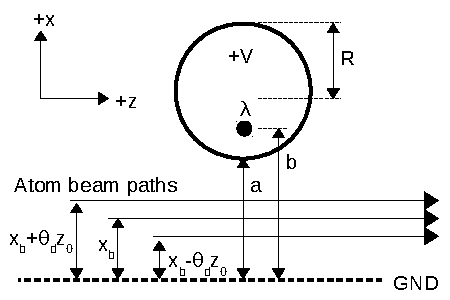
\includegraphics[width=\linewidth,keepaspectratio]{EDiagram1.pdf}
\caption{\label{EDiagram}Diagram showing the dimensions that describe the static electric fields created by the pillars and by the phase choppers. The circle represents the cross-section of a metal pillar or charged wire with radius $R$ held at voltage $V$. The GND line represents the ground plane, which may by physical (in the case of the choppers) or virtual (in the case of the pillars), a distance $a$ away from the pillar edge. The parameter $b$ is the distance between the ground plane and the effective line charge within the pillar. The atom beam center is a distance $x_b$ away from the ground plane, and the different interferometer arms are separated from their neighbors by a distance $\theta_d z_0$. $a$ and $R$ dimensions for the pillars and phase choppers are given in Table \ref{tableDimensions}.}
\end{figure}

Both the pillars and the phase choppers are described by the geometry shown in \figref{EDiagram}, and have electric fields given by
\begin{align}
	\vec{E}(x,z) = \frac{\lambda}{2\pi\epsilon_0}
	\left[	
		\frac{x-b}{(x-b)^2+z^2} - \frac{x+b}{(x+b)^2+z^2}
	\right] \hat{x} \nonumber \\
	+ 
	\left[	
		\frac{z}{(x-b)^2+z^2} - \frac{z}{(x+b)^2+z^2}
	\right] \hat{z}
	\label{EPillars}
\end{align}
The effective line charge density
\begin{align}
	\lambda = 2\pi\epsilon_0V\ln^{-1}
	\left(
		\frac{a+R+b}{a+R-b}
	\right)
	\label{lambda}
\end{align}
exists a distance $b = a\sqrt{1+2R/a}$ away from the ground plane, where $a$ is the distance between the ground plane and the closest cylinder edge, $R$ is the cylinders' radius, and $\hat{x}$ and $\hat{z}$ are shown in \figref{EDiagram}.

When atoms enter an electric field, their total energy changes by $U_{\mathrm{Stark}} = -\frac{1}{2}\alpha|\vec{E}|^2$; thus the electric field represents a region of lower potential energy for that atoms.
Since $U_{\mathrm{Stark}} \ll E_{\mathrm{kinetic}}$ in our experiment, we can use the WKB approximation along with the Residue Theorem to compute the total phase accumulated by an atom travelling through the field.
Even though an atom in the beam may be misaligned by an angle of up to $10^{-3}$ with the different fields' ground planes, we can approximate that atoms always travel parallel to the beamline distance $x_b$ away from the ground plane. Therefore, the accumulated phase along one path for a component of an atomic de Broglie wave is
\begin{align}
	\Phi(v,x) = 
	\frac{1}{\hbar v} \int_{-\infty}^{\infty} \frac{1}{2} \alpha |\vec{E}|^2 dz =	
	\frac{\lambda^2 \alpha}{\pi \epsilon_0^2 \hbar v}
	\left( \frac{b}{b^2-x_b^2} \right)
	\label{accumPhasePillars}
\end{align}

The differential phase shifts for the interferometers on the + and - sides of the beamline (see \figref{IFMDiagram}) are
\begin{align}
	\Delta\Phi_{\vec{E},+}(v,x_b) = \Phi(v, x_b+\theta_d z_0) - \Phi(v, x_b) \nonumber \\
	\Delta\Phi_{\vec{E},-}(v,x_b) = \Phi(v, x_b) - \Phi(v, x_b-\theta_d z_0)
	\label{deltaPhasePillars}
\end{align}
where $\theta_d z_0$ is the lateral separation between classical paths in the interferometer. 

\subsection{II.b. Velocity Measurement}

The atoms in the beam do not all have the same velocity, so the electric fields do not apply the same phase to each atom on a given path.
We observe the average phase and contrast of an ensemble of atoms diffracting to first order on either side of the beamline with velocity distribution $P(v)$. 
We model $P(v)$ as a Gaussian distribution
\begin{align}
	P(v)dv = \frac{v_r}{v_0\sqrt{2\pi}}e^{-\frac{v_r^2(v-v_0)^2}{2v_0^2}}
	\label{PvelGaussian}
\end{align}
where $v_0$ is the mean velocity and $v_r = v_0/\sigma_v$ is a measure of the distribution's sharpness. It is worth noting that the velocity distribution for a supersonic atom beam is better described by a $v^3$-weighted Gaussian distribution
\cite{Berman1997}. However, either distribution can be used in our analysis to parametrize the typical high-$v_0$, high-$v_r$ velocity distributions of our atom beam without changing our polarizability result. Importantly, since $v_0$ is the average velocity in a Gaussian but not in a $v^3$-weighted Gaussian, we choose to use the former for our data analysis in order to simplify the error analysis. 

%Without modelling the beam this way, we would report $\alpha$ 1.5\% too high.

\begin{figure}
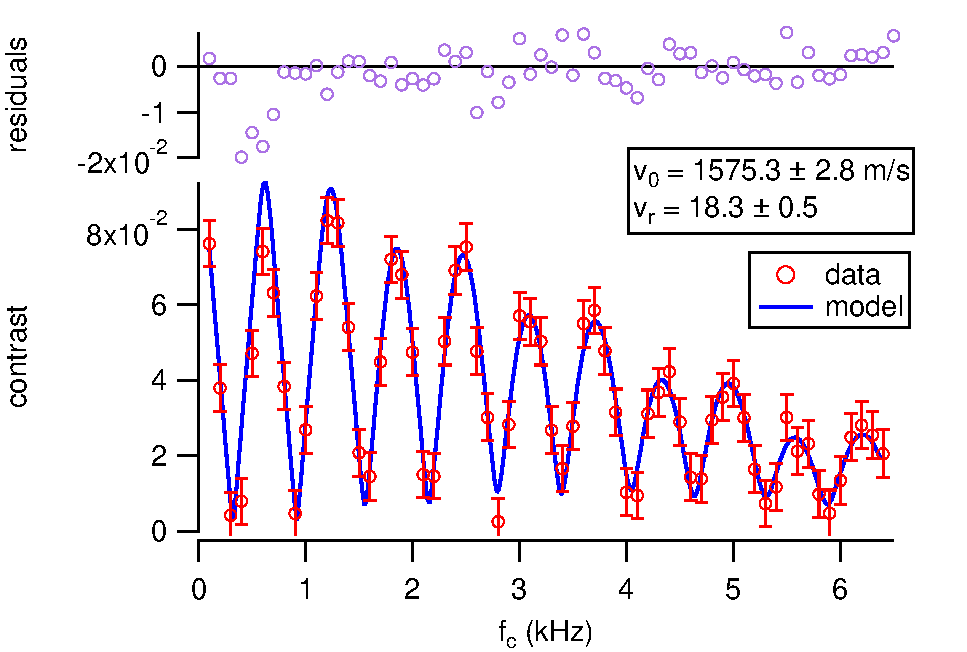
\includegraphics[width=\linewidth,keepaspectratio]{CvCF_150420_o.pdf}
\caption{\label{CvCFExample}(Color online) An example of a measurement of contrast vs. phase chopper frequency for a Cs beam. We fit a model to these data that has $v_0$ and $v_r$ as fit parameters in order to measure the velocity distribution.}
\end{figure}

To measure $v_0$ and $v_r$, we use phase choppers \cite{Holmgren2011,Hromada2014}. Each phase chopper is a charged wire about 1 mm away from a physical ground plane (see Table \ref{tableDimensions} for phase chopper dimensions). Chopper 1 is between the first two gratings and chopper 2 is a distance $z_{c1,c2} = 1269.3 \pm 0.25$ mm downstream of chopper 1, between the last two gratings (see \figref{IFMDiagram}). The voltages on the choppers' wires and the distances between the beam and the choppers' ground planes are chosen such that chopper 1 shifts the ensemble's average phase by $+\pi$ and chopper 2 shifts it by $-\pi$. 

When we pulse the choppers on and off at frequency $f_c$, an atom may receive a net phase shift of $\pm\pi$ or $0$ depending on its velocity and when they passed through the first chopper. 
Holmgren \etalspace gives an intuitive explanation of how
we measure contrast $C$ vs $f_c$ to determine $v_0$ and $v_r$ \cite{Holmgren2011} (\figref{CvCFExample} shows an example of $C/C_{\mathrm{ref}}$ vs $f_c$ data). Hromada \etalspace later improved upon Holmgren \etal's model of $C$ vs $f_c$ \cite{Hromada2014}.

Using phase choppers allows us to measure $v_0$ and $v_r$ for Cs without needing to obtain resolved diffraction. In our earlier work, we measured $v_0$ and $v_r$ by scanning the detector's $x$ position to observe the diffraction pattern through grating 1 \cite{Holmgren2010}. However, since the diffraction angle for Cs is so small, we would need a thinner detector wire and thinner collimating slits to resolve diffraction peaks, which would in turn reduce statistical precision.

Hromada \etalspace describes how the thickness and divergence of the beam determines the likelihood for atoms of certain velocities to be detected \cite{Hromada2014}.
The thickness and divergence is defined by the finite widths of the collimating slits $w_1$ and $w_2$, the finite width of the detector $w_{\mathrm{det}}$, and the detector's offset from the beamline in the $x$ direction $\Delta x_{\mathrm{det}}$.
The phase and contrast we observe with our detector is that of an ensemble of atoms with different velocities, different incident positions on the grating 1, and different incident angles on the grating 1.
Uncertainties in $w_1$, $w_2$, $w_{\mathrm{det}}$, and $\Delta x_{\mathrm{det}}$ are more significant for beams that are physically wider. 
In K beams, which have higher $\theta_d$ and lower $v_r$ (i.e. a wider velocity distribution), more of the lower-velocity atoms in the distribution miss the detector. Therefore, uncertainties in the aforementioned quanitities have a higher bearing on how we model the average velocity of \textit{detected} atoms.
Ignoring this component of the analysis causes a systematic increase in measured $v_0$ by 0.05\% and $v_r$ by 10\% for a typical K beam, which corresponds to a 0.15\% error in $\ak$.

Hromada \etalspace also describes how inequality between $L_1$ and $L_2$ causes systematic errors \cite{Hromada2014}. 
When $\Delta L = L_1 - L_2$ is nonzero, the different paths in the interferometer interfere the most not at the third grating but at some other $z$ position within the beamline.
This effect magnifies the projection of the interference fringes onto the third grating. We summarize this geometric magnification with the separation phase shift:
\begin{align}
	\dphisepj = \frac{2\pi}{d_g}
	\left(
		\theta_{inc} + \frac{j}{2}\theta_d
	\right) \Delta L
	\label{phiSep}
\end{align}
where $j=1$ and $j=-1$ represent the interferometers on the + and - side of the beamline, respectively, and $\theta_{\mathrm{inc}}$ is the incident angle on grating 1. 
To reduce systematic error in our $v_0$ and $v_r$ measurements, 
we must be able to measure $\Delta L$ and set it equal to zero.

\begin{figure}
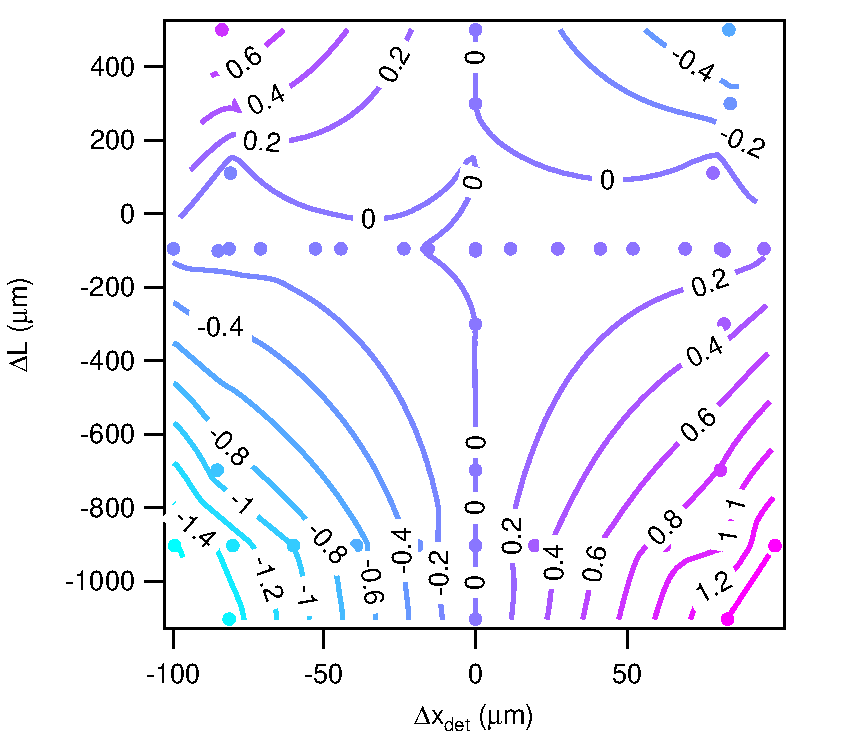
\includegraphics[width=\linewidth,keepaspectratio]{phaseVsdxDetdL_141202.pdf}
\caption{\label{PhaseVsThings}(Color online)
Data showing the phase of the interference fringes as a function of $\Delta x_{\mathrm{det}}$ and $\Delta L$. $\Phi$ vs $\Delta x_{\mathrm{det}}$ is a line with slope proportional to $\Delta L$. 
}
\end{figure}

\eqnref{phiSep} implies that uncertainty in $\Delta L$ is more significant for beams with larger $\theta_d$, such as K beams.
Also, because $\dphisepj$ has a component proportional to $\theta_{\mathrm{inc}}$, uncertainty in $\Delta L$ is more significant for more divergent beams.
Furthermore, as $|\Delta L|$ increases, the measured $v_0$ and $v_r$ become more dependent on $w_1$, $w_2$, $w_{\mathrm{det}}$, and $\Delta x_{\mathrm{det}}$. Accordingly, we set $\Delta L = 0$ to reduce contributions to systematic uncertainty from uncertainty in those sources. 
\eqnref{phiSep} implies that interferometers on either side of the beamline receive opposite phase shifts. 
Therefore, by moving the the detector in the $\pm x$ direction, we  observe linear changes in $\Phi$ per $\Delta x_{\mathrm{det}}$ with slope proportional to $\Delta L$.
\figref{PhaseVsThings} shows data that demonstrates this effect.
We set $\Delta L$ to 0 $\pm$ 30 $\mu$m by finding the $\Delta L$ for which d$\Phi/$d$x_{\mathrm{det}} = 0$.

If the interferometer grating bars are significantly non-vertical, it can become necessary to consider the phase shift induced by the component of gravitational acceleration in the plane of the interferometer, which is given by
\begin{align}
	\dphiaccel = \frac{\pi g\sin({\theta_g})(L_1+L_2)^2}{2d_g v^2}
	\label{phiAccel}
\end{align}
where $\theta_g$ is the tilt of the grating bars with respect to vertical. 
Our interferometer's $|\theta_g|$ never exceeded 2.3 mrad. If we were to neglect this portion of the analysis, we would report $v_0$ incorrectly by up to 0.015\% and $v_r$ incorrectly by up to 0.25\%.

\begin{figure}
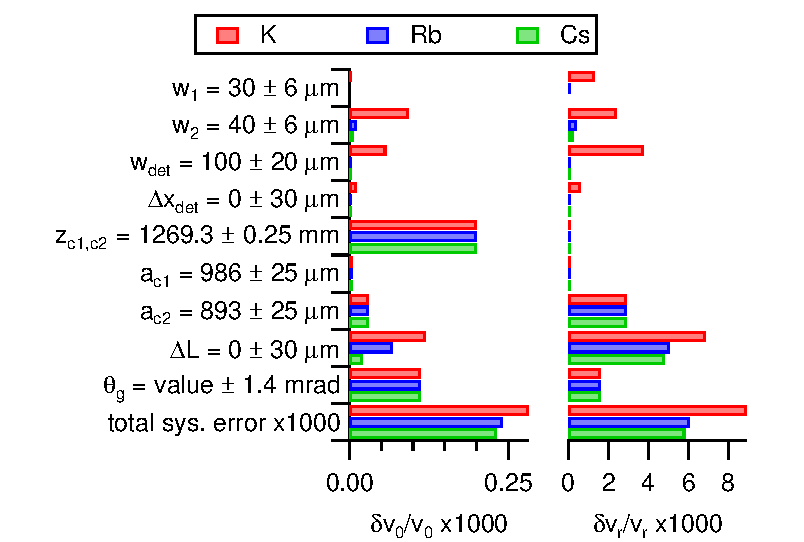
\includegraphics[width=\linewidth,keepaspectratio]{displayVelErrors.pdf}
\caption{\label{velError}(Color online) Systematic uncertainty budget for measurements of $v_0$ and $v_r$ for our Cs, Rb, and K beams. $a_{ci}$ is the width of phase chopper $i$. A nominal value for $\theta_g$ is not listed because $\theta_g$ changed from -2.37 mrad to 1.73 mrad toward the end of the experiment.}
\end{figure}

The uncertainty budget for $v_0$ and $v_r$ measurements is given in \figref{velError}. 
The measured values of $v_0$ and $v_r$ also have statistical uncertainty in addition to uncertainty in the fit of measured $C/C_{\mathrm{ref}}(f_c)$ to the model. Uncertainty in the measurement of $\Delta\Phi = \Phi_{c1,\mathrm{on}} - \Phi_{\mathrm{ref}}$ leads to uncertainty in $A_{ci}$, which in turn propagates forward as additional uncertainty in $v_0$ and $v_r$. The total statistical uncertainty in measured $v_0$ and $v_r$ is roughly $10\times$ larger than the total systematic uncertainty.

\begin{figure}
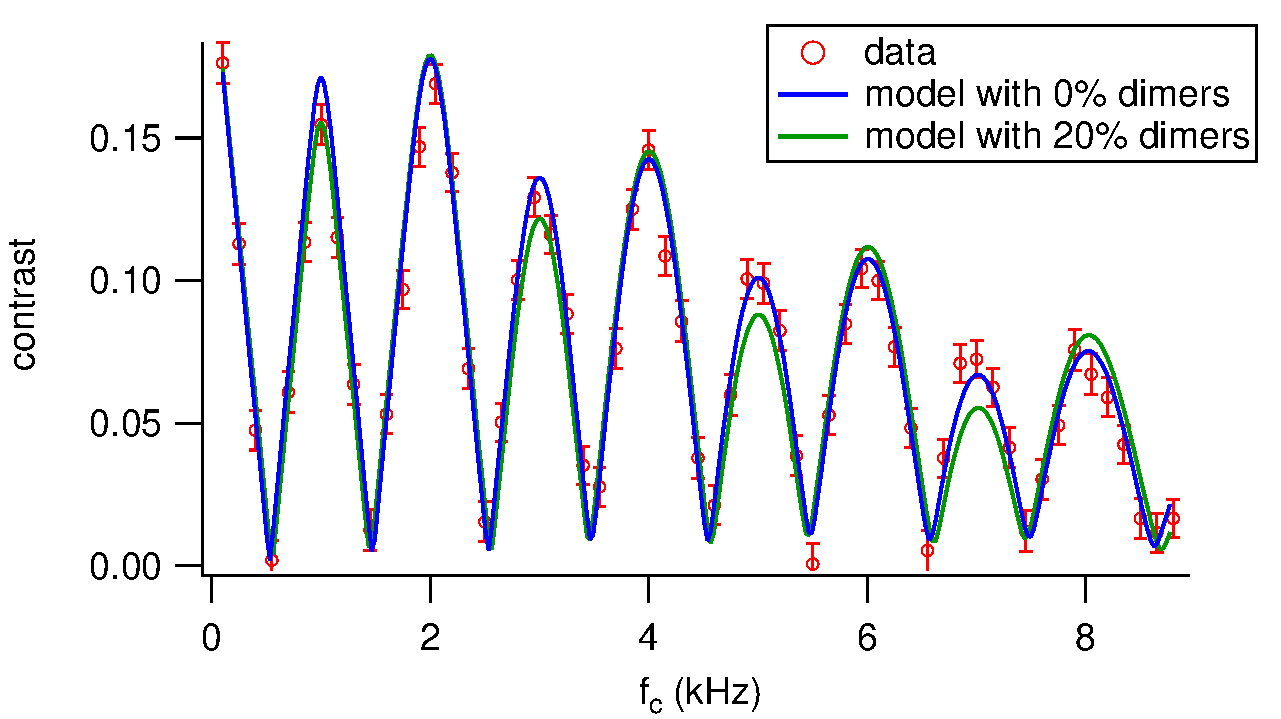
\includegraphics[width=\linewidth,keepaspectratio]{CvCFDimers_140924.pdf}
\caption{\label{CvCFDimers}(Color online) This figure illustrates how changing the fraction of dimers in the beam, $f_d$, affects the model of $C$ vs $f_c$. The data (red) was first fit with a model (blue) in which the dimer fraction $r_d$ was a fit parameter. The model best fit the data when $r_d = 0$. The model in green shows what $C$ vs $f_c$ would look like if $v_0$ and $v_r$ were the same but $r_d$ were equal to 0.2.}
\end{figure}

Atoms in an alkali metal gas have a small probability of forming homonuclear dimers, which have different polarizabilities than monomers. 
We were able to use the phase choppers data along with Molof \etal's dimer-to-monomer polarizability ratios \cite{Molof1974} to put an upper bound on the fraction of dimers in the beam. We inserted the dimer fraction $r_d$ as an additional fit parameter to $C$ vs $f_c$.
The covariances among $r_d$, $v_0$, and $v_r$ are all low--changing $r_d$ affects the model of $C$ vs $f_c$ in a way that is different from how changing $v_0$ or $v_r$ affects the model (see \figref{CvCFDimers}). 
Using this method, we determined that $r_d = 0 \pm 2\%$. We added this possibility of beams with 2\% dimers to the error analysis of polarizability data, discussed in the next section.


\subsection{II.c. Polarizability Measurement}

To measure the Cs, Rb, and K polarizability, we use two parallel, oppositely charged, $1/2$-inch-diameter pillars. The pillars are mounted to a single, rigid support structure so that a 3999.7 $\pm$ 1.0 $\mu$m gap exists between them. A motor moves the support structure in the $\pm x$ direction, and a length gauge monitors the structure's $x$ position. 
We begin a polarizability measurement with the assembly positioned such that the beam passes through the gap between the pillars near one of the edges.
We take 25 sec of data each with the electric field on and off, and then move the pillars about 400 $\mu$m so that the beam approaches the other edge of the gap. We repeat this 9 times to 
observe the phase shift $\Delta\Phi = \Phi_{\mathrm{pillars,on}} - \Phi_{\mathrm{ref}}$ applied by the pillars as a function $x_b$ (see an example in \figref{dPvMPExample}). 
When the electric field is off, we observe the reference phase $\Phi_{\mathrm{ref}}$ and reference contrast $C_{\mathrm{ref}}$ given by 
\begin{align}
	C_{\mathrm{ref}}e^{\Phi_{\mathrm{ref}}} = 
		C_0e^{\Phi_0} \frac{1}{2} \sum_{j=-1,1}
		\int_{v=0}^{\infty} P(v)
		e^{\dphisag(v)} 
		dv
	\label{CPPolesRef}
\end{align}
The Sagnac phase, $\dphisag$, is described in our previous work \cite{Holmgren2010}.
$C_0$ is the contrast that would be observed in the absence of $\dphisag(v)$, and $\Phi_0$ is an arbitrary phase constant.
When the field is on, we instead observe
\begin{align}
	C_{\textrm{pillars,on}}e^{\Phi_{\textrm{pillars,on}}} = 
		\nonumber \\
		C_0e^{\Phi_0}		
		\frac{1}{2} \sum_{j=-1,1}
		\int_{v=0}^{\infty} P(v)
		e^{
			\Delta\Phi_{\vec{E},j}(v,x_b) + 
			\dphisag(v)
		} 
		dv
	\label{CPPolesEOn}
\end{align}
We fit a model to $\Delta\Phi = \Phi_{\mathrm{pillars,on}} - \Phi_{\mathrm{ref}}$ vs $x_b$, as shown in \figref{dPvMPExample}. The fit parameters of that model are $\alpha$ and the pillars position for which the phase shift is null $x_{b0}$ (i.e. the location of the virtual ground plane). 

In our earlier work, we used one pillar next to a grounded plate instead of two pillars forming a virtual ground plane \cite{Holmgren2010}. We would measure $x_b$ by eclipsing the beam with the grounded plate, and there were systematic errors associated with this procedure. 
Our new pillars assembly eliminates those systematic errors, and having $x_{b0}$ be a fit parameter of the $\Delta\Phi$ vs $x_b$ model adds an insignificant amount of statistical uncertainty to the determined $\alpha$.

\begin{figure}
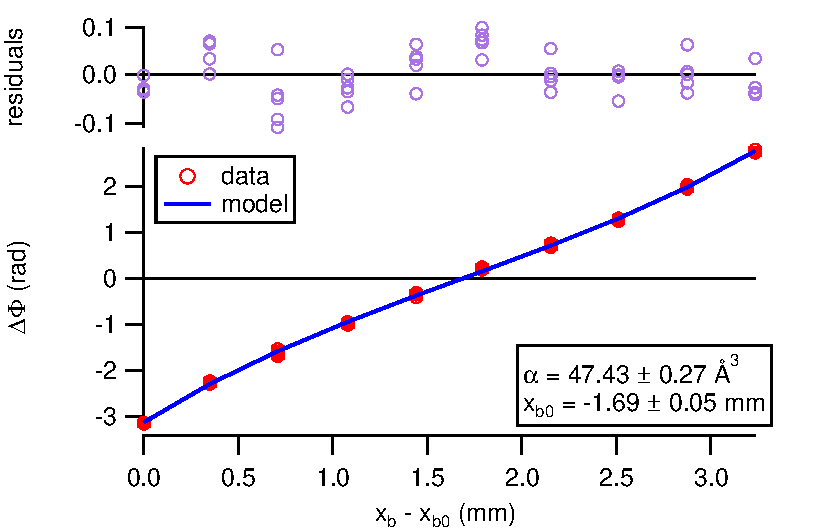
\includegraphics[width=\linewidth,keepaspectratio]{dPvMP_150327_q.pdf}
\caption{\label{dPvMPExample}(Color online) An example of a measurement of phase shift vs $x$ position of the pillars for a Rb beam. The two fit parameters used to fit the model to these data are polarizability $\arb$ and the pillars' position at which the phase shift is null $x_{b0}$.}
\end{figure}

\begin{figure}
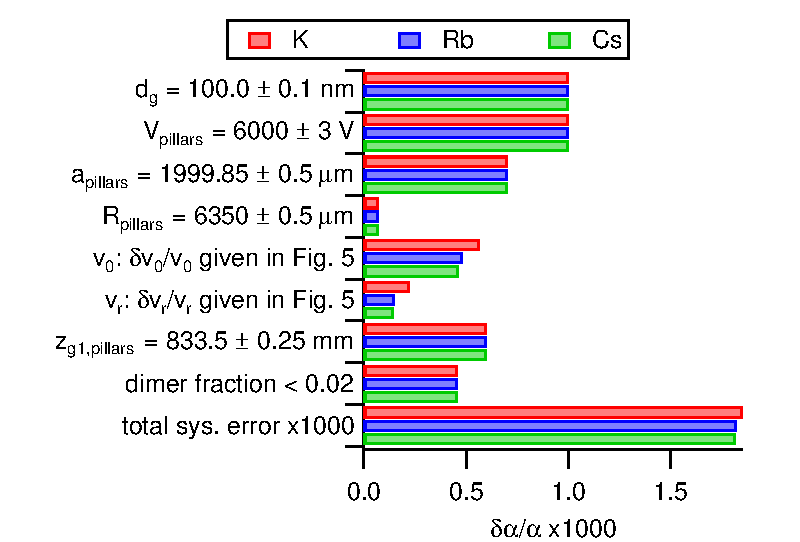
\includegraphics[width=\linewidth,keepaspectratio]{displayPolErrors.pdf}
\caption{\label{polError}(Color online) Systematic uncertainty budget for polarizability measurements for our Cs, Rb, and K beams.
The uncertainties in knowledge of $v_0$ and $v_r$ are propagated forward from \figref{velError}.}
\end{figure}

The systematic uncertainty budget for the absolute polarizability measurements is shown in \figref{polError}. 
We constructed the new pillars using steel rods, the widths of which were accurately known to $1 \mu \text{m}$. This reduced the uncertainty in $R_{\mathrm{pillars}}$ by about a factor of 10.
We reduced the uncertainty in the $V_{\mathrm{pillars}}$ by a factor of 3 by independently calibrating our voltage supplies. We also measured $a_{\mathrm{pillars}}$ to 0.5 $\mu$m accuracy rather than 1 $\mu$m accuracy and measured $z_{g1,\mathrm{pillars}}$ to 1/4 mm accuracy rather than 2 mm accuracy. 

Our $\theta_g$ was always close enough to zero such that we did not need to consider $\dphiaccel$ in our polarizability data analysis--we would only need to consider $\dphiaccel$ if $|\theta_g|$ exceeded 23 mrad.
Even if we do consider $\dphisep$ along with $\dphisag$ in Eqns \ref{CPPolesRef} and \ref{CPPolesEOn}, we find that our 30$\mu$m uncertainty in $\Delta L$ corresponds to only 0.002\% uncertainty in $\alpha$.
Additionally, we found that modeling the beam's thickness and divergence was unnecessary for analysis of polarizability data if $\Delta L = 0$, though it becomes increasingly important as $|\Delta L|$ increases.
Therefore $w_1$, $w_2$, $w_{\mathrm{det}}$, and $\Delta x_{\mathrm{det}}$ do not appear in the polarizability analysis error budget.

Considering second order diffraction in our models does not change reported $v_0$ by more than 0.005\%, $v_r$ by 0.2\%, and $\alpha$ by 0.01\%.

\subsection{II.d. Data Analysis}

\begingroup
\begin{table}
\caption{\label{schedule}A typical sequence of measurements during a day of data acquisition. The $+x$ direction is arbitrarily chosen--the important aspect is that we spend an equal amount of time scanning the pillars in each direction so as to minimize possible systematic errors. This sequence of eight measurements is repeated for as long as we choose to acquire data. We end the data acquisition by repeating the first four measurements.}
\begin{center}
\begin{tabular}{l l}
\hline
\hline
Type of data acquired & Duration \\
\hline
contrast vs chopping freq. & 7m 5s \\
chopper 1 phase & 3m 45s \\
chopper 2 phase & 3m 45s\\
contrast vs chopping freq. & 7m 5s \\
$\Delta\Phi$ vs pillars position ($+x$ direction) \sspace & 8m 45s \\
$\Delta\Phi$ vs pillars position ($-x$ direction) & 8m 45s \\
$\Delta\Phi$ vs pillars position ($+x$ direction) & 8m 45s \\
$\Delta\Phi$ vs pillars position ($-x$ direction) & 8m 45s \\
\hline
\hline
\end{tabular}
\end{center}
\end{table}
\endgroup

A typical sequence of measurements is shown in Table \ref{schedule}.
We measure the velocity distribution twice between every four scans of the pillars across the beam, and calibrate the phase choppers between each pair of velocity measurements.

We linearly interpolate between $v_0$ and $v_r$ measurements to obtain the velocity distribution at the time of each scan of the pillars.
We also tried using cubic spline interpolation and Gaussian Process Regression to interpolate between $v_0$ and $v_r$ measurements. Using these different methods changed our reported polarizabilities by no more than 0.008\%, which is small compared to our statistical uncertainties.

\section{III. Results and Discussion}

Table \ref{tableAbs} shows our absolute measurements of Cs, Rb, and K polarizability and their statistical and systematic uncertainties. The statistical uncertainty reported is the standard error of the mean.

\begingroup
\begin{table}
\caption{\label{tableAbs}Absolute measurements of Cs, Rb, and K static, ground-state polarizabilities.}
\begin{center}
\begin{tabular}{llll}
\hline\hline
Atom \sspace & avg $v_0$ (m/s) \sspace & avg $v_r$ \sspace & $\alpha$(stat.)(sys.) ($\AAA^3$) \\
\hline
Cs & 1585 & 19.8 & $\polCs$ \\
Rb & 1890 & 22.9 & $\polRb$ \\
K  & 2113 & 13.2 & $\polK$ \\
\hline\hline
\end{tabular}
\end{center}
\end{table}
\endgroup

Table \ref{tableRatio} shows our ratio measurement results. 
Because we used the same apparatus for each absolute measurement,
most of the systematic uncertainties mentioned in \figref{velError} and \figref{polError} among measurements.
These correlated uncertainties do not contribute toward systematic error of the ratios. 
Uncertainties in $w_1$, $w_2$, $w_{\mathrm{det}}$, and $\Delta L$ contribute differently to systematic uncertainty in $\acs$, $\arb$, and $\ak$ measurements, and therefore also contribute toward the systematic uncertainties of the ratios.
The ratios' statistical uncertainties are almost 20 times higher than the ratios' systematic uncertainties.

\begingroup
\begin{table}
\caption{\label{tableRatio}Ratio measurements of Cs, Rb, and K static, ground-state polarizabilities. The systematic errors in each ratio, which arise from the fact that the systematic errors in different measurements are not perfectly correlated, are negligible compared to the statistical errors.}
\begin{center}
\begin{tabular}{lll}
\hline\hline
Ratio \ssspace \ssspace & Value(stat.) \sspace & Sys. Err. \\
\hline
$\acs/\ak$  & $\ratCsK$ & $4\cdot 10^{-5}$  \\
$\acs/\arb$ & $\ratCsRb$ & $5\cdot 10^{-6}$ \\
$\arb/\ak$  & $\ratRbK$ & $3\cdot 10^{-5}$ \\
\hline\hline
\end{tabular}
\end{center}
\end{table}
\endgroup

\subsection{III.a. Comparisons With Other Experimental and Theoretical Polarizabilities}

\begin{figure*}
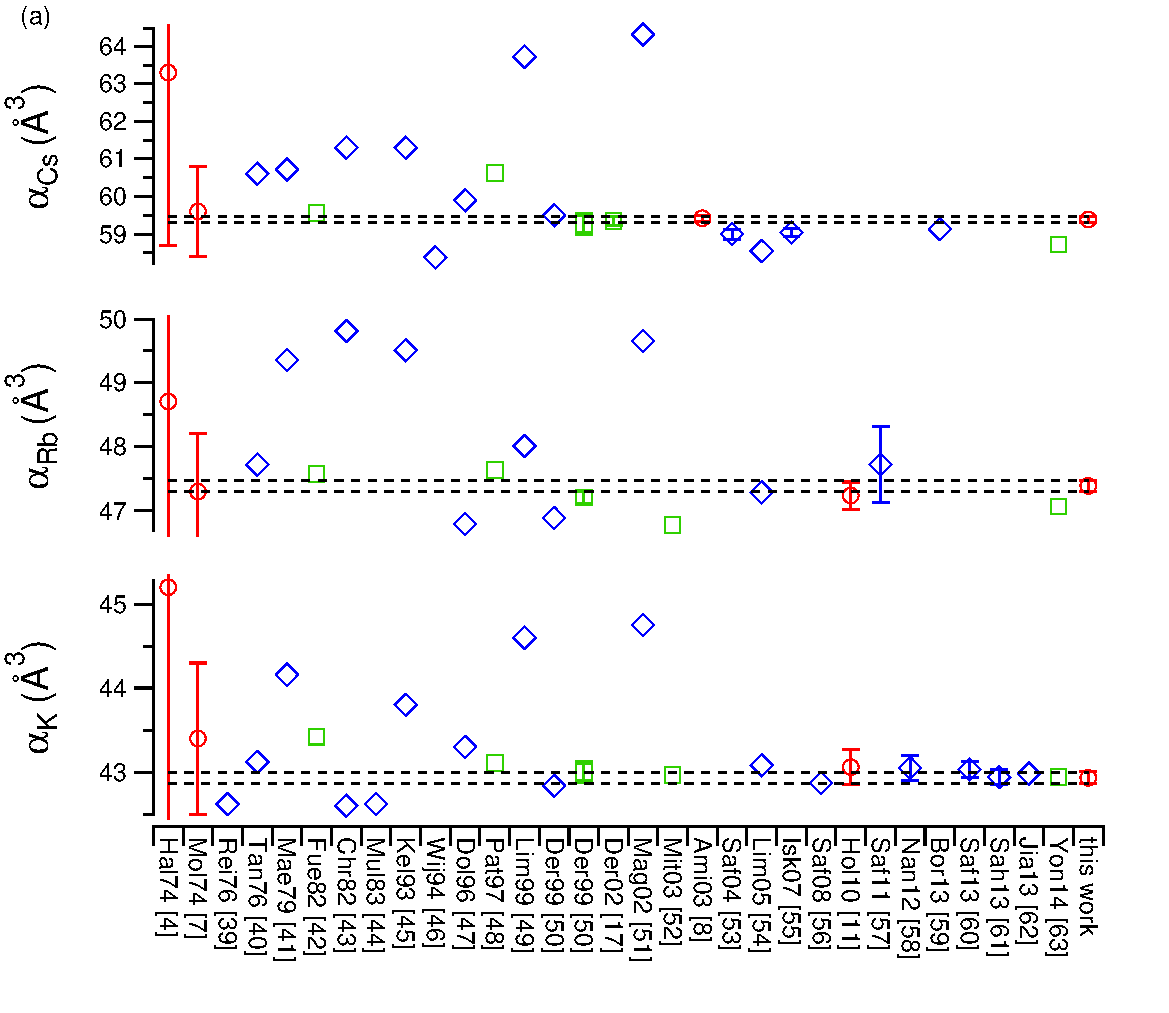
\includegraphics[width=0.60\linewidth,keepaspectratio]{displayAbsComps.pdf}
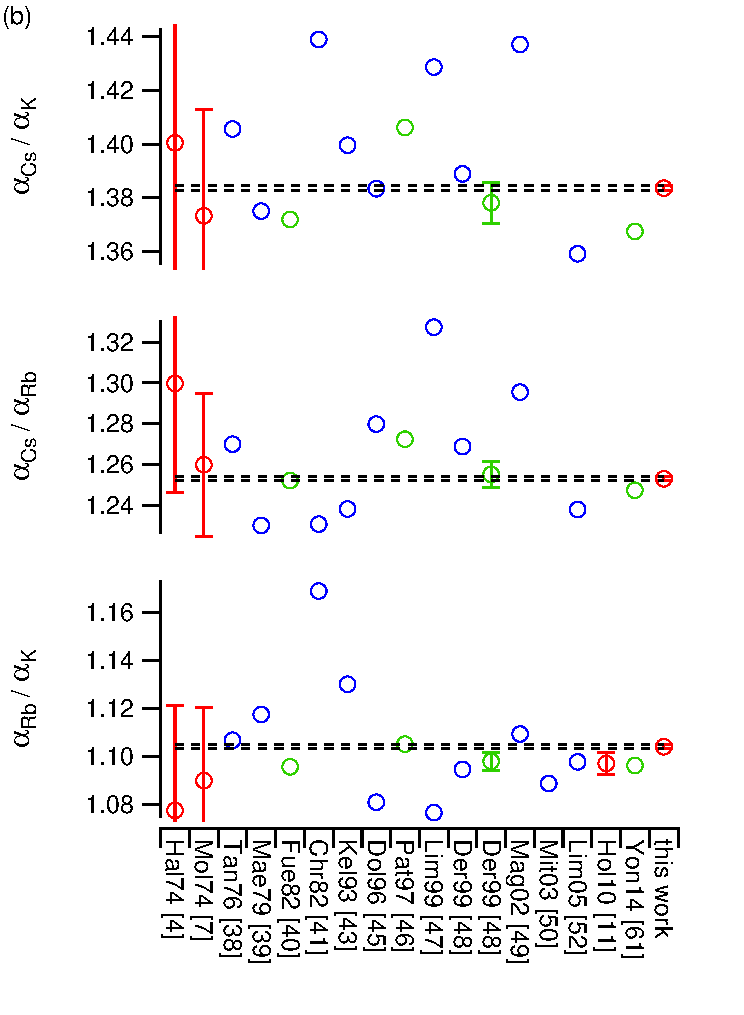
\includegraphics[width=0.38\linewidth,keepaspectratio]{displayRatComps.pdf}

\includegraphics[width=0.55\linewidth,keepaspectratio]{displayCompsLegend.pdf}
\caption{\label{comparisons}(Color online) Our absolute measurements (left) and ratio measurements (right) compared with other measurements, \textit{ab initio} calculations, and semi-empirical calculations 
\cite{Molof1974a,Hall1974,Tang1976,Reinsch1976,Kutzelnigg1978,
Christiansen1982,Fuentealba1999,Muller1984,Kello1993,VanWijngaarden1994,
Dolg1996,Patil1997,Derevianko1998,Magnier2002,Derevianko2001,
Amini2003,Mitroy2003,Safronova2004,Lim2005,Safronova2008,
Holmgren2010,Safronova2011,Nandy2012,Jiang2013,Sahoo2013,
Safronova2013,Borschevsky2013,Y.-B.2014}.
The references are represented on the x-axis by the first three letters of the first author's last name followed by the year of publication. For the semi-empirical calculations: Reference Fue82 used semi-empirical pseudopotentials \cite{Fuentealba1999}, Pat97 used experimentally-determined energy levels \cite{Patil1997}, Der99 used experimentally-determined electric dipole transition matrix elements \cite{Derevianko1998}, and Yon14 used semi-empirical core polarization potentials \cite{Y.-B.2014}.}.
\end{figure*}

\begin{figure}
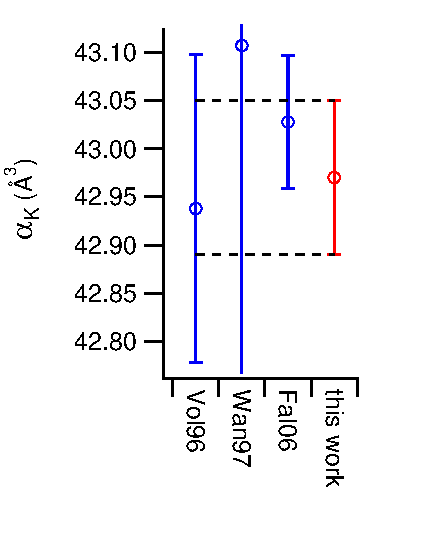
\includegraphics[width=0.49\linewidth,keepaspectratio,valign=t]{displayKMisc.pdf}
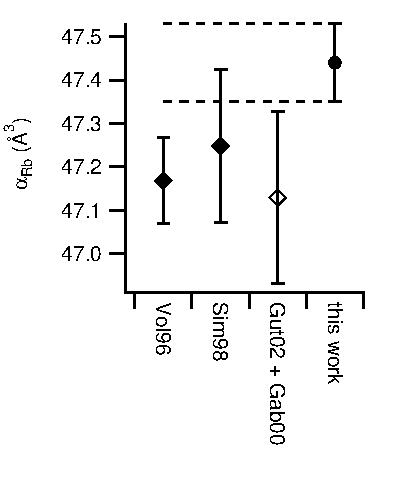
\includegraphics[width=0.49\linewidth,keepaspectratio,valign=t]{displayRbMisc.pdf}
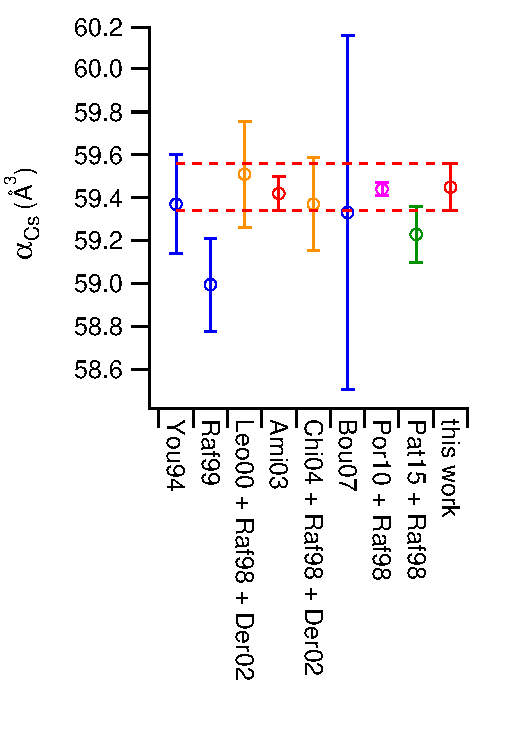
\includegraphics[width=0.620\linewidth,keepaspectratio,valign=t]{displayCsMisc.pdf}
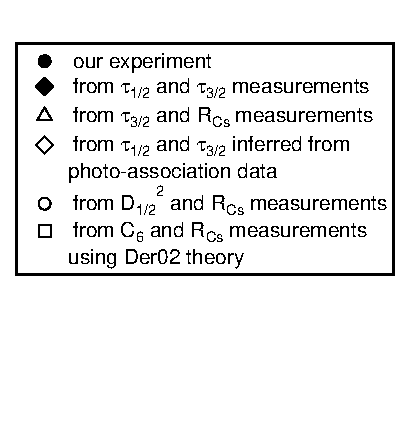
\includegraphics[width=0.365\linewidth,keepaspectratio,valign=t]{displayMiscLegend.pdf}
\caption{\label{comparisonsMisc}(Color online) Comparisons of our measured polarizabilities and Amini and Gould's $\acs$ measurement \cite{Amini2003} to polarizabilities derived from measured lifetimes and lifetime ratios,
\cite{Young1994,Rafac1999,Bouloufa2007,Falke2006a,Volz2006,Simsarian1998,Wang1997,Rafac1998}, 
lifetimes inferred from photo-association data
\cite{Gabbanini2000,Gutterres2002},
theoretical $D^2$ values
\cite{Porsev2010},
and van der Waals $C_6$ measurements
\cite{Leo2000,Chin2004,Derevianko2001}.}
\end{figure}

\figref{comparisons} compares our polarizability measurements with theoretical calculations, semi-empirical calculations, and experimental measurements subsequent to and including Molof \etal's and Hall \etal's 1974 measurements \cite{Molof1974a,Hall1974}. Our absolute measurements are consistent with all previous absolute measurements. 
In particular, our $\acs$ measurement agrees very well with Amini and Gould's $\acs$ measurement (shown again in \figref{comparisonsMisc}) \cite{Amini2003}. Amini and Gould's $\acs$ measurement, in addition to being dramatic improvement in precision since the previous measurement by Molof \etalspace \cite{Molof1974a}, is the only polarizability measurement using the fountain method. The fact that we obtained a very similar $\acs$ as Amini and Gould with a very different apparatus goes a long way toward validating both methods.

\figref{comparisons} also compares our ratios to other theoretical, semi-empirical, and experimental ratios. Our ratios are also consistent with all previous ratio measurements.

\subsection{III.b. Comparisons With Polarizabilities Derived From Other Quantities}

Static polarizabilities can be related to electric dipole transition matrix elements, state lifetimes, oscillator strengths, and van der Waals coefficients. We will describe those relations and compare our $\alpha$ measurements to $\alpha$ values derived from recent calculations and high-precision measurements of those quantities; those comparisons are shown in \figref{comparisonsMisc}.

\begingroup
\begin{table}
\caption{\label{tableOmegaRes}We use the following ground-state to first-excited-state transition frequencies and the following residual polarizabilities $\alpha_r$.
$N = 6$ for Cs, $N = 5$ for Rb, and $N = 4$ for K.
Frequencies were calculated using transition wavelengths reported in NIST's Atomic Spectra Database \cite{NIST}.
The sources for $\alpha_r$ values are cited next to the values in the table.}
\begin{center}
\begin{tabularx}{\linewidth}{lXXl}
\hline\hline
Atom$\quad$ & $\omega_{Ns_{1/2}-Np_{1/2}}$ ($10^{15}$ Hz) & $\omega_{Ns_{1/2}-Np_{3/2}}$ ($10^{15}$ Hz) & $\alpha_r$ ($\AAA^3$) \\
\hline
Cs & 2.1056 & 2.2099 & 2.481(16) \cite{Derevianko2001} \\
Rb & 2.3694 & 2.4142 & 1.562(89) \cite{Safronova2006} \\
K  & 2.4459 & 2.4568 & 0.925(45) \cite{Safronova2006} \\
\hline\hline
\end{tabularx}
\end{center}
\end{table}
\endgroup

The polarizability (in volume units) of an atom in state $i$ can be written in terms of state lifetimes as
\begin{align}
	\alpha_i = \frac{3c^3}{2} \sum_{k\neq i} 
	\frac{1}{\tau_{ki} \omega_{ik}^4} \frac{g_k}{3g_i}
	+ \alpha_r
	\label{polFromLifetimes}
\end{align}
where $\tau_{ki}$ is the lifetime associated with spontaneous decay from state $k$ to $i$, $\omega_{ik}$ is the transition frequency between states $i$ and $k$, and $g_n = 2J_n+1$ is the degeneracy factor for state $n$. In our case, state $i$ is the ground state. 
The residual polarizability $\alpha_r$ is the sum of the terms not explicitly included in the sum, the polarizability of the core electrons, and a correction accounting for correlations between core and valence electrons.
We only explicitly sum over $Ns_{1/2}-Np_{1/2}$ and $Ns_{1/2}-Np_{3/2}$ transitions, where $N=6$ for Cs, $N=5$ for Rb, and $N=4$ for K, and we abbreviate the lifetimes associated with those transitions to $\tau_{1/2}$ and $\tau_{3/2}$.
In our calculations, we use the $\omega_{0k}$ and $\alpha_r$ values indicated in Table \ref{tableOmegaRes}.
\figref{comparisonsMisc} shows polarizabilities calculated using measurements of $\tau_{1/2}$ and $\tau_{3/2}$
\cite{Young1994,Rafac1999,Bouloufa2007,Falke2006a,Volz2006,Simsarian1998,Wang1997}.
\figref{comparisonsMisc} also shows $\acs$ calculated from 
values of $\tau_{1/2,\mathrm{Rb}}$ and $\tau_{3/2,\mathrm{Rb}}$ inferred in 2002 by Gutterres \etalspace from photo-association data taken in 2000 by Gabbanini \etalspace \cite{Gabbanini2000,Gutterres2002}.
Additionally, Rafac and Tanner measured the ratio of Cs electric dipole transition matrix elements \cite{Rafac1998}
\begin{align}
	\rcs = \frac
	{\left|\brakett{6s_{1/2}}{\hat{D}}{6p_{3/2}}\right|^2}
	{\left|\brakett{6s_{1/2}}{\hat{D}}{6p_{1/2}}\right|^2}
	\label{polFromLifetimes}
\end{align}
which we can use to deduce a ratio of lifetimes
\begin{align}
	\frac{\tau_{1/2}}{\tau_{3/2}} = \frac{\rcs}{2} \left( \frac{\omega_{3/2}}{\omega_{1/2}} \right)^3
	\label{RafacRLifetimes}
\end{align}
We can use this lifetimes ratio with Patterson \etal's 2015 measurement of $\tau_{3/2,\mathrm{Cs}}$ to report $\acs$ \cite{Patterson2015}.

We can write $\alpha_i$ in terms of the electric dipole transition matrix elements as
\begin{align}
	\alpha_i = \frac{e^2}{12 \pi \epsilon_0 a_0^4} \sum_{k\neq i}	
	\frac{\left|\brakett{i}{\hat{D}}{k}\right|^2}{\hbar\omega_{ik}}	
	+ \alpha_r
	\label{polFromMatrixElements}
\end{align}
where $a_0$ is the Bohr radius. 
As before, we only explicitly consider the $Ns_{1/2}-Np_{1/2}$ and $Ns_{1/2}-Np_{3/2}$ matrix elements, 
where $Ns_{1/2}$ is the ground state.
We use $\rcs$ along with Porsev \etal's 2010 calculation of $D_{1/2,\mathrm{Cs}}^2 = 20.334$ (in atomic units) to report polarizability \cite{Rafac1998,Porsev2010}.

In 2002, Derevianko and Porsev demonstrated a method for obtaining values of $D_{1/2,\mathrm{Cs}}^2$ from Cs van der Waals $C_6$ coefficients \cite{Derevianko2001}. \figref{comparisonsMisc} includes $\alpha$ values derived using experimental Cs $C_6$ measurements in conjunction with Derevianko and Porsev's method and $\rcs$ \cite{Leo2000,Chin2004,Derevianko2001,Rafac1998}.

\subsection{III.c. Other Atomic Properties Derived From Our Polarizability Measurements}

\begingroup
\begin{table}
\caption{\label{tableR}Matrix element ratios $\mathcal{R} = D_{3/2}^2/D_{1/2}^2$ for Cs, Rb, and K. The sources for the ratios are cited next to the values in the table.}
\begin{center}
\begin{tabular}{lll}
\hline\hline
Atom \sspace & $\mathcal{R}$ \\
\hline
Cs & 1.9809(9) & \cite{Rafac1998} \\
Rb & 1.99219(3) & \cite{Leonard2015} \\
K  & 2.000(4) & \cite{Holmgren2012} \\
\hline\hline
\end{tabular}
\end{center}
\end{table}
\endgroup

\begingroup
\begin{table}
\caption{\label{tableMisc}Matrix elements, lifetimes, oscillator strengths, line strengths, and van der Waals $C_6$ coefficients calculated from our polarizability measurements.
We used $\mathcal{R}$ values from Table \ref{tableR}. The matrix elements, line strengths, and $C_6$ coefficient are expressed in atomic units, while the lifetimes are expressed in SI units.
$\delta_{\alpha}$, $\delta_{\mathcal{R}}$, and $\delta_{\alpha_r}$ represent the uncertainties in the values due to uncertainty in $\alpha$, $\mathcal{R}$, and $\alpha_r$, respectively. $\delta_{\mathrm{tot}}$ is the total uncertainty in the value.}
\begin{center}
\begin{tabular}{lllllll}
\hline\hline
Quantity & Atom & Value & $\delta_{\alpha}$ & $\delta_{\mathcal{R}}$ & $\delta_{\alpha_r}$ & $\delta_{\mathrm{tot}}$ \\
\hline
$|D_{1/2}|$ 		& Cs & 4.103 & (4) & (3) & (2) & (5) \\
 					& Rb & 4.244 & (4) & ($<1$) & (4) & (6) \\
 					& K  & 4.510 & (4) & (1) & (1) & (4) \\ \hline
$|D_{3/2}|$ 		& Cs & 5.803 & (6) & (2) & (3) & (7) \\
 					& Rb & 5.990 & (6) & ($<1$) & (6) & (8) \\
 					& K  & 6.348 & (6) & ($<1$) & (1) & (6) \\ \hline
$\tau_{1/2}$ (ns) 	& Cs & 26.78 & (5) & (4) & (3) & (7) \\
 					& Rb & 27.53 & (5) & ($<1$) & (5) & (8) \\
 					& K  & 34.73 & (7) & (1) & (1) & (7) \\ \hline
$\tau_{3/2}$ (ns) 	& Cs & 26.42 & (5) & (2) & (3) & (6) \\
 					& Rb & 26.13 & (5) & ($<1$) & (5) & (7) \\
 					& K  & 30.33 & (6) & ($<1$) & (1) & (6) \\ \hline
$f_{1/2}$ 			& Cs & 0.332 & (1) & ($<1$) & ($<1$) & (1) \\
 					& Rb & 0.344 & (1) & ($<1$) & (1) & (1) \\
 					& K  & 0.345 & (1) & ($<1$) & ($<1$) & (1) \\ \hline
$f_{3/2}$ 			& Cs & 0.667 & (1) & ($<1$) & (1) & (2) \\
 					& Rb & 0.699 & (1) & ($<1$) & (1) & (2) \\
 					& K  & 0.718 & (1) & ($<1$) & ($<1$) & (1) \\ \hline
$S_{1/2}$ 			& Cs & 16.83 & (3) & (2) & (2) & (4) \\
 					& Rb & 18.01 & (4) & ($<1$) & (3) & (5) \\
 					& K  & 20.34 & (4) & (1) & (1) & (4) \\ \hline
$S_{3/2}$ 			& Cs & 33.68 & (6) & (2) & (4) & (8) \\
 					& Rb & 35.89 & (7) & ($<1$) & (7) & (10) \\
 					& K  & 40.30 & (8) & (1) & (1) & (8) \\ \hline
$C_6$ 				& Cs & 6881 & (23) & (3) & (3) & (24) \\ \hline
\hline
\end{tabular}
\end{center}
\end{table}
\endgroup

Finally, we use our polarizability measurements to report matrix elements $|D|$, lifetimes, oscillator strengths, and line strengths. We also emply Derevianko and Porsev's method to report a Cs van der Waals $C_6$ coefficient.
In these calculations, we use residual polarizabilities $\alpha_r$ from Table \ref{tableOmegaRes} and matrix element ratios $\mathcal{R}$
from Table \ref{tableR}.
To report matrix elements and lifetimes, we use \eqnref{polFromMatrixElements} and \eqnref{polFromLifetimes}. $\alpha_i$ is given in terms of oscillator strengths $f_{ik}$ as 
\begin{align}
	\alpha_i = \frac{e^2}{4 \pi \epsilon_0 m}
	\sum_{k \neq i}
	\frac{f_{ik}}{w_{ik}^2}
	+ \alpha_r
	\label{polFromOscStr}
\end{align}
where $m$ is the electron mass. 
$\alpha_i$ is also given in terms of line strengths as
\begin{align}
	\alpha_i = \frac{1}{6\pi\epsilon_0\hbar} 
	\sum_{k \neq i} 
	\frac{S_{ki}}{g_i\omega_{ik}}
	+ \alpha_r
	\label{polFromLineStr}
\end{align}

We note that our $\left|D_{1/2,\mathrm{Cs}}\right|$ value agrees very well with the theoretical $\left|D_{1/2,\mathrm{Cs}}\right|$ calculated by Porsev \etalspace in 2010 for the purpose of interpreting PNC data \cite{Porsev2010}.

\begingroup
\begin{table}
\caption{\label{tableR}Excited state polarizabilities $\alpha_{Np_{1/2}}$, where $N = 6$ for Cs, $N = 5$ for Rb, and $N = 4$ for K. The values were calculated using our measurements and $\alpha_{Np_{1/2}} - \alpha_{Ns_{1/2}}$ measurements \cite{Hunter1991,Miller1994}.}
\begin{center}
\begin{tabular}{l l l}
\hline\hline
Atom \sspace & $\alpha_{Np_{1/2}}$ \\
\hline
Cs & 196.87(11) \\
Rb & 120.38(9) \\
K  & 89.96(8) \\
\hline\hline
\end{tabular}
\end{center}
\end{table}
\endgroup



Finally, we use our measurements together with recent measurements of Cs, Rb, and K $\alpha_{Np_{1/2}} - \alpha_{Ns_{1/2}}$ \cite{Hunter1991,Miller1994} to report excited state polarizabilities $\alpha_{Np_{1/2}}$ with better than 0.09\% uncertainty. 
These results are also shown in Table \ref{tableMisc}.

\section{IV. Outlook}

We are currently exploring ways to measure the polarizability of either Li or metastable He, the polarizabilities of which can be easily calculated. By measuring $\acs/\alpha_{\mathrm{He*}}$ or $\acs/\alpha_{\mathrm{Li}}$, we could report an absolute measurement of $\acs$ with precision comparable to that of the ratios reported here for the benefit of PNC research. Such a measurement would also act as a calibration of the measurements presented in this work, because it would be independent of systematic errors that may affect our absolute measurements.

We are also exploring electron-impact ionization schemes for atom detection, which would allow us to detect a much broader range of atoms and molecules. Our Langmuir-Taylor only allows us to detect alkali metals and some alkaline-Earth metals \cite{Delhuille2002}. Installing a new, "universal" detector would allow us to broaden the scope of atom interferometry as a precision measurement tool. 

This work is supported by NSF Grant No. 1306308 and a NIST PMG. M.D.G. and R.T. are grateful for NSF GRFP Grant No. DGE-1143953 for support. 


%\bibliography{references}
\bibliography{library}

\end{document}  